\documentclass{article}\usepackage[]{graphicx}\usepackage[]{xcolor}
% maxwidth is the original width if it is less than linewidth
% otherwise use linewidth (to make sure the graphics do not exceed the margin)
\makeatletter
\def\maxwidth{ %
  \ifdim\Gin@nat@width>\linewidth
    \linewidth
  \else
    \Gin@nat@width
  \fi
}
\makeatother

\definecolor{fgcolor}{rgb}{0.345, 0.345, 0.345}
\newcommand{\hlnum}[1]{\textcolor[rgb]{0.686,0.059,0.569}{#1}}%
\newcommand{\hlstr}[1]{\textcolor[rgb]{0.192,0.494,0.8}{#1}}%
\newcommand{\hlcom}[1]{\textcolor[rgb]{0.678,0.584,0.686}{\textit{#1}}}%
\newcommand{\hlopt}[1]{\textcolor[rgb]{0,0,0}{#1}}%
\newcommand{\hlstd}[1]{\textcolor[rgb]{0.345,0.345,0.345}{#1}}%
\newcommand{\hlkwa}[1]{\textcolor[rgb]{0.161,0.373,0.58}{\textbf{#1}}}%
\newcommand{\hlkwb}[1]{\textcolor[rgb]{0.69,0.353,0.396}{#1}}%
\newcommand{\hlkwc}[1]{\textcolor[rgb]{0.333,0.667,0.333}{#1}}%
\newcommand{\hlkwd}[1]{\textcolor[rgb]{0.737,0.353,0.396}{\textbf{#1}}}%
\let\hlipl\hlkwb

\usepackage{framed}
\makeatletter
\newenvironment{kframe}{%
 \def\at@end@of@kframe{}%
 \ifinner\ifhmode%
  \def\at@end@of@kframe{\end{minipage}}%
  \begin{minipage}{\columnwidth}%
 \fi\fi%
 \def\FrameCommand##1{\hskip\@totalleftmargin \hskip-\fboxsep
 \colorbox{shadecolor}{##1}\hskip-\fboxsep
     % There is no \\@totalrightmargin, so:
     \hskip-\linewidth \hskip-\@totalleftmargin \hskip\columnwidth}%
 \MakeFramed {\advance\hsize-\width
   \@totalleftmargin\z@ \linewidth\hsize
   \@setminipage}}%
 {\par\unskip\endMakeFramed%
 \at@end@of@kframe}
\makeatother

\definecolor{shadecolor}{rgb}{.97, .97, .97}
\definecolor{messagecolor}{rgb}{0, 0, 0}
\definecolor{warningcolor}{rgb}{1, 0, 1}
\definecolor{errorcolor}{rgb}{1, 0, 0}
\newenvironment{knitrout}{}{} % an empty environment to be redefined in TeX

\usepackage{alltt}
\usepackage[sc]{mathpazo}
\renewcommand{\sfdefault}{lmss}
\renewcommand{\ttdefault}{lmtt}
\usepackage[T1]{fontenc}
\usepackage{geometry}
\geometry{verbose,tmargin=2.5cm,bmargin=2.5cm,lmargin=2.5cm,rmargin=2.5cm}
\setcounter{secnumdepth}{2}
\setcounter{tocdepth}{2}
\usepackage[unicode=true,pdfusetitle,
 bookmarks=true,bookmarksnumbered=true,bookmarksopen=true,bookmarksopenlevel=2,
 breaklinks=false,pdfborder={0 0 1},backref=false,colorlinks=false]
 {hyperref}
\hypersetup{
 pdfstartview={XYZ null null 1}}

\makeatletter
%%%%%%%%%%%%%%%%%%%%%%%%%%%%%% User specified LaTeX commands.
\renewcommand{\textfraction}{0.05}
\renewcommand{\topfraction}{0.8}
\renewcommand{\bottomfraction}{0.8}
\renewcommand{\floatpagefraction}{0.75}

\makeatother
\IfFileExists{upquote.sty}{\usepackage{upquote}}{}
\begin{document}



\title{\title{\title{\title{\title{\title{\title{\title{\title{\title{}}}}}}}}}}



\maketitle
The results below are generated from an R script.

\begin{knitrout}
\definecolor{shadecolor}{rgb}{0.969, 0.969, 0.969}\color{fgcolor}\begin{kframe}
\begin{alltt}
\hlcom{# Assignment Week4_02}
\hlcom{# Couto, Maria}
\hlcom{# 07/01/2023}

\hlkwd{setwd}\hlstd{(}\hlstr{"C:/Users/ait0s/OneDrive/Documents/Github/dsc520/data"}\hlstd{)}

\hlcom{# Load Housing Dataset}
\hlkwd{library}\hlstd{(readxl)}
\hlstd{housedf} \hlkwb{<-} \hlkwd{read_excel}\hlstd{(}\hlstr{"week-6-housing.xlsx"}\hlstd{)}

\hlcom{# Use the apply function on a variable in your dataset}
\hlkwd{library}\hlstd{(plyr)}
\hlkwd{library}\hlstd{(dplyr)}
\end{alltt}


{\ttfamily\noindent\itshape\color{messagecolor}{\#\# \\\#\# Attaching package: 'dplyr'}}

{\ttfamily\noindent\itshape\color{messagecolor}{\#\# The following objects are masked from 'package:plyr':\\\#\# \\\#\# \ \ \ \ arrange, count, desc, failwith, id, mutate, rename, summarise, summarize}}

{\ttfamily\noindent\itshape\color{messagecolor}{\#\# The following objects are masked from 'package:stats':\\\#\# \\\#\# \ \ \ \ filter, lag}}

{\ttfamily\noindent\itshape\color{messagecolor}{\#\# The following objects are masked from 'package:base':\\\#\# \\\#\# \ \ \ \ intersect, setdiff, setequal, union}}\begin{alltt}
\hlkwd{apply}\hlstd{(housedf,}\hlnum{2}\hlstd{,length)}
\end{alltt}
\begin{verbatim}
##                Sale Date               Sale Price              sale_reason 
##                    12865                    12865                    12865 
##          sale_instrument             sale_warning                 sitetype 
##                    12865                    12865                    12865 
##                addr_full                     zip5                  ctyname 
##                    12865                    12865                    12865 
##               postalctyn                      lon                      lat 
##                    12865                    12865                    12865 
##           building_grade square_feet_total_living                 bedrooms 
##                    12865                    12865                    12865 
##          bath_full_count          bath_half_count          bath_3qtr_count 
##                    12865                    12865                    12865 
##               year_built           year_renovated           current_zoning 
##                    12865                    12865                    12865 
##                sq_ft_lot                prop_type              present_use 
##                    12865                    12865                    12865
\end{verbatim}
\begin{alltt}
\hlcom{# Use the aggregate function on a variable in your dataset}

\hlstd{housedf} \hlkwb{<-} \hlstd{housedf} \hlopt \hlkwd{rename_at}\hlstd{(}\hlnum{1}\hlstd{,}\hlopt{~}\hlstr{'sale_date'}\hlstd{)}
\hlstd{housedf} \hlkwb{<-} \hlstd{housedf} \hlopt \hlkwd{rename_at}\hlstd{(}\hlnum{2}\hlstd{,}\hlopt{~}\hlstr{'sale_price'}\hlstd{)}

\hlkwd{aggregate}\hlstd{(sale_price}\hlopt{~}\hlstd{ctyname,housedf,mean)}
\end{alltt}
\begin{verbatim}
##     ctyname sale_price
## 1   REDMOND   644803.2
## 2 SAMMAMISH   972480.3
\end{verbatim}
\begin{alltt}
\hlkwd{aggregate}\hlstd{(sale_price}\hlopt{~}\hlstd{ctyname} \hlopt{+} \hlstd{bedrooms, housedf, median)}
\end{alltt}
\begin{verbatim}
##      ctyname bedrooms sale_price
## 1    REDMOND        0     953830
## 2    REDMOND        1     960000
## 3    REDMOND        2     392000
## 4  SAMMAMISH        2     434000
## 5    REDMOND        3     507000
## 6  SAMMAMISH        3     581000
## 7    REDMOND        4     659650
## 8  SAMMAMISH        4     820000
## 9    REDMOND        5     722750
## 10 SAMMAMISH        5    1070500
## 11   REDMOND        6     665000
## 12 SAMMAMISH        6    1230000
## 13   REDMOND        7     522450
## 14   REDMOND        9     581500
## 15   REDMOND       10     450000
## 16   REDMOND       11    1825000
\end{verbatim}
\begin{alltt}
\hlkwd{aggregate}\hlstd{(sale_price}\hlopt{~}\hlstd{year_built,housedf,median)}
\end{alltt}
\begin{verbatim}
##     year_built sale_price
## 1         1900   427500.0
## 2         1903   430000.0
## 3         1905   620000.0
## 4         1906   550000.0
## 5         1909     1070.0
## 6         1910   150000.0
## 7         1912   580000.0
## 8         1913   457500.0
## 9         1914   835000.0
## 10        1915   228150.0
## 11        1916   350000.0
## 12        1918  1200000.0
## 13        1919   476800.0
## 14        1920   522500.0
## 15        1922   386675.0
## 16        1923   300000.0
## 17        1924   636500.0
## 18        1925   402000.0
## 19        1926   255000.0
## 20        1927  1282500.0
## 21        1928   520000.0
## 22        1929  1242500.0
## 23        1930   360000.0
## 24        1931   168828.5
## 25        1932   487031.0
## 26        1933   465000.0
## 27        1934   782500.0
## 28        1935   339000.0
## 29        1936   430000.0
## 30        1937   338750.0
## 31        1938  1675500.0
## 32        1939   520000.0
## 33        1940   520000.0
## 34        1941   460000.0
## 35        1942   392000.0
## 36        1943   425000.0
## 37        1944   335626.5
## 38        1945   323250.0
## 39        1946   637500.0
## 40        1947   401000.0
## 41        1948   605500.0
## 42        1949   427350.0
## 43        1950   360000.0
## 44        1951   515000.0
## 45        1952   500000.0
## 46        1953   434000.0
## 47        1954   530000.0
## 48        1955   482500.0
## 49        1956   550000.0
## 50        1957   475000.0
## 51        1958   440000.0
## 52        1959   427500.0
## 53        1960   448000.0
## 54        1961   516252.0
## 55        1962   435000.0
## 56        1963   460000.0
## 57        1964   461200.0
## 58        1965   470000.0
## 59        1966   465000.0
## 60        1967   479950.0
## 61        1968   439975.0
## 62        1969   429725.0
## 63        1970   391000.0
## 64        1971   442000.0
## 65        1972   543500.0
## 66        1973   551017.0
## 67        1974   539500.0
## 68        1975   520000.0
## 69        1976   495000.0
## 70        1977   475000.0
## 71        1978   485000.0
## 72        1979   520000.0
## 73        1980   520000.0
## 74        1981   520000.0
## 75        1982   527000.0
## 76        1983   520000.0
## 77        1984   540000.0
## 78        1985   560000.0
## 79        1986   555000.0
## 80        1987   608000.0
## 81        1988   744350.0
## 82        1989   750000.0
## 83        1990   767500.0
## 84        1991   765000.0
## 85        1992   609250.0
## 86        1993   685000.0
## 87        1994   736250.0
## 88        1995   650000.0
## 89        1996   675000.0
## 90        1997   720500.0
## 91        1998   752500.0
## 92        1999   860000.0
## 93        2000   715000.0
## 94        2001   595000.0
## 95        2002   567000.0
## 96        2003   595000.0
## 97        2004   620000.0
## 98        2005   622495.0
## 99        2006   672000.0
## 100       2007   656000.0
## 101       2008   645470.0
## 102       2009   616580.5
## 103       2010   617750.0
## 104       2011   626675.0
## 105       2012   663900.0
## 106       2013   705907.0
## 107       2014   853990.0
## 108       2015   940445.0
## 109       2016   904480.5
\end{verbatim}
\begin{alltt}
\hlkwd{distinct}\hlstd{(housedf,ctyname)}
\end{alltt}
\begin{verbatim}
## # A tibble: 3 x 1
##   ctyname  
##   <chr>    
## 1 REDMOND  
## 2 <NA>     
## 3 SAMMAMISH
\end{verbatim}
\begin{alltt}
\hlcom{# Use the plyr function on a variable in your dataset – }
\hlcom{# more specifically, I want to see you split some data, }
\hlcom{# perform a modification to the data, and then bring it back together}

\hlkwd{distinct}\hlstd{(housedf,ctyname)}
\end{alltt}
\begin{verbatim}
## # A tibble: 3 x 1
##   ctyname  
##   <chr>    
## 1 REDMOND  
## 2 <NA>     
## 3 SAMMAMISH
\end{verbatim}
\begin{alltt}
\hlstd{housedf_v2} \hlkwb{<-}\hlkwd{mutate}\hlstd{(housedf,}\hlkwc{ctyname} \hlstd{=} \hlkwd{if_else}\hlstd{(}\hlkwd{is.na}\hlstd{(ctyname),}
                                              \hlstr{"City_Unkown"}\hlstd{,ctyname))}
\hlkwd{distinct}\hlstd{(housedf_v2,ctyname)}
\end{alltt}
\begin{verbatim}
## # A tibble: 3 x 1
##   ctyname    
##   <chr>      
## 1 REDMOND    
## 2 City_Unkown
## 3 SAMMAMISH
\end{verbatim}
\begin{alltt}
\hlstd{housedf_v2} \hlkwb{<-} \hlkwd{mutate}\hlstd{(housedf_v2,}\hlkwc{Price_per_sqft} \hlstd{=}
                       \hlstd{sale_price}\hlopt{/}\hlstd{square_feet_total_living)}
\hlkwd{colnames}\hlstd{(housedf_v2)}
\end{alltt}
\begin{verbatim}
##  [1] "sale_date"                "sale_price"               "sale_reason"             
##  [4] "sale_instrument"          "sale_warning"             "sitetype"                
##  [7] "addr_full"                "zip5"                     "ctyname"                 
## [10] "postalctyn"               "lon"                      "lat"                     
## [13] "building_grade"           "square_feet_total_living" "bedrooms"                
## [16] "bath_full_count"          "bath_half_count"          "bath_3qtr_count"         
## [19] "year_built"               "year_renovated"           "current_zoning"          
## [22] "sq_ft_lot"                "prop_type"                "present_use"             
## [25] "Price_per_sqft"
\end{verbatim}
\begin{alltt}
\hlcom{# Check distributions of the data}
\hlkwd{library}\hlstd{(ggplot2)}
\hlkwd{theme_set}\hlstd{(}\hlkwd{theme_minimal}\hlstd{())}

\hlkwd{aggregate}\hlstd{(Price_per_sqft}\hlopt{~}\hlstd{ctyname,housedf_v2,median)}
\end{alltt}
\begin{verbatim}
##       ctyname Price_per_sqft
## 1 City_Unkown       245.5763
## 2     REDMOND       251.3587
## 3   SAMMAMISH       244.5009
\end{verbatim}
\begin{alltt}
\hlkwd{ggplot}\hlstd{(housedf_v2,} \hlkwd{aes}\hlstd{(Price_per_sqft))} \hlopt{+}
  \hlkwd{geom_histogram}\hlstd{(}\hlkwc{bins} \hlstd{=} \hlnum{100}\hlstd{,}\hlkwc{color} \hlstd{=} \hlstr{"black"}\hlstd{,} \hlkwc{fill} \hlstd{=} \hlstr{"yellow"}\hlstd{)} \hlopt{+}
  \hlkwd{ggtitle}\hlstd{(}\hlstr{"Housing Data"}\hlstd{)} \hlopt{+}
  \hlkwd{labs}\hlstd{(}\hlkwc{x} \hlstd{=}\hlstr{"Price Per Square Feet"}\hlstd{,} \hlkwc{y}\hlstd{=}\hlstr{"Count of Homes Sold"}\hlstd{)}
\end{alltt}
\end{kframe}

{\centering 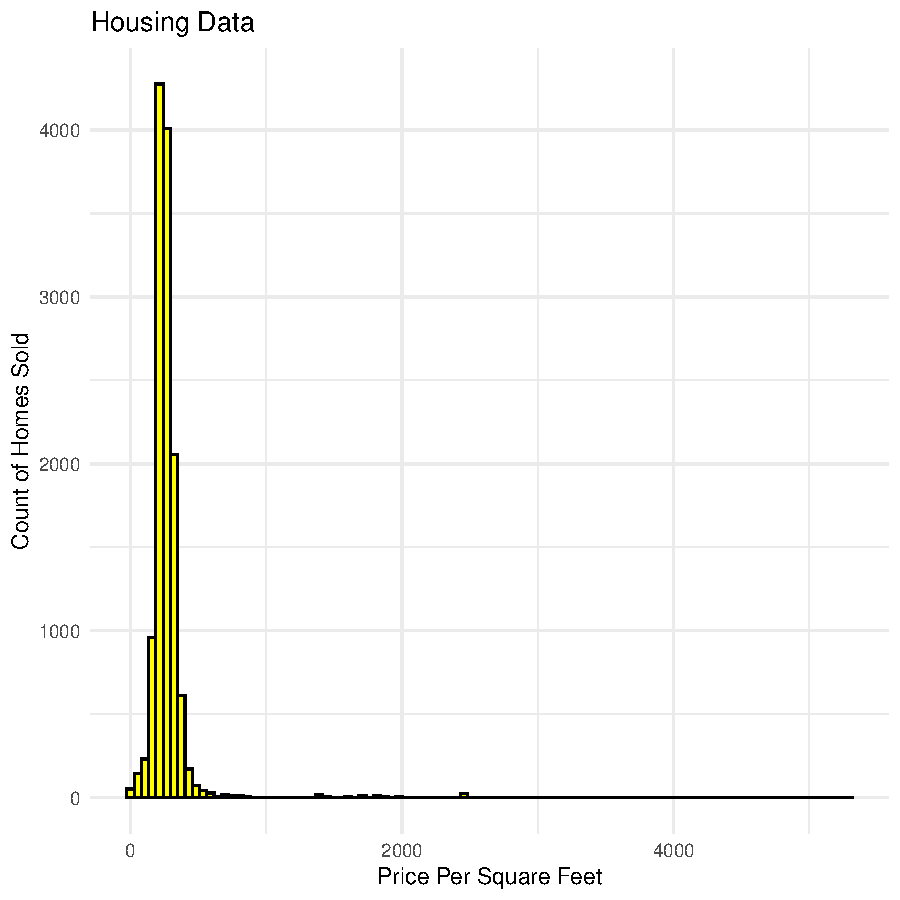
\includegraphics[width=.6\linewidth]{figure/assignment-04-02-Couto-Maria-Rnwauto-report-1} 

}


\begin{kframe}\begin{alltt}
\hlcom{# Identify if there are any outliers}

\hlkwd{ggplot}\hlstd{(housedf_v2,} \hlkwd{aes}\hlstd{(}\hlkwc{x}\hlstd{=sale_price,}\hlkwc{y}\hlstd{=square_feet_total_living,}
                       \hlkwc{colour}\hlstd{=ctyname))} \hlopt{+}
  \hlkwd{geom_point}\hlstd{(}\hlkwc{size} \hlstd{=} \hlnum{2}\hlstd{)} \hlopt{+}
  \hlkwd{xlab}\hlstd{(}\hlstr{"Sales Price"}\hlstd{)}
\end{alltt}
\end{kframe}

{\centering 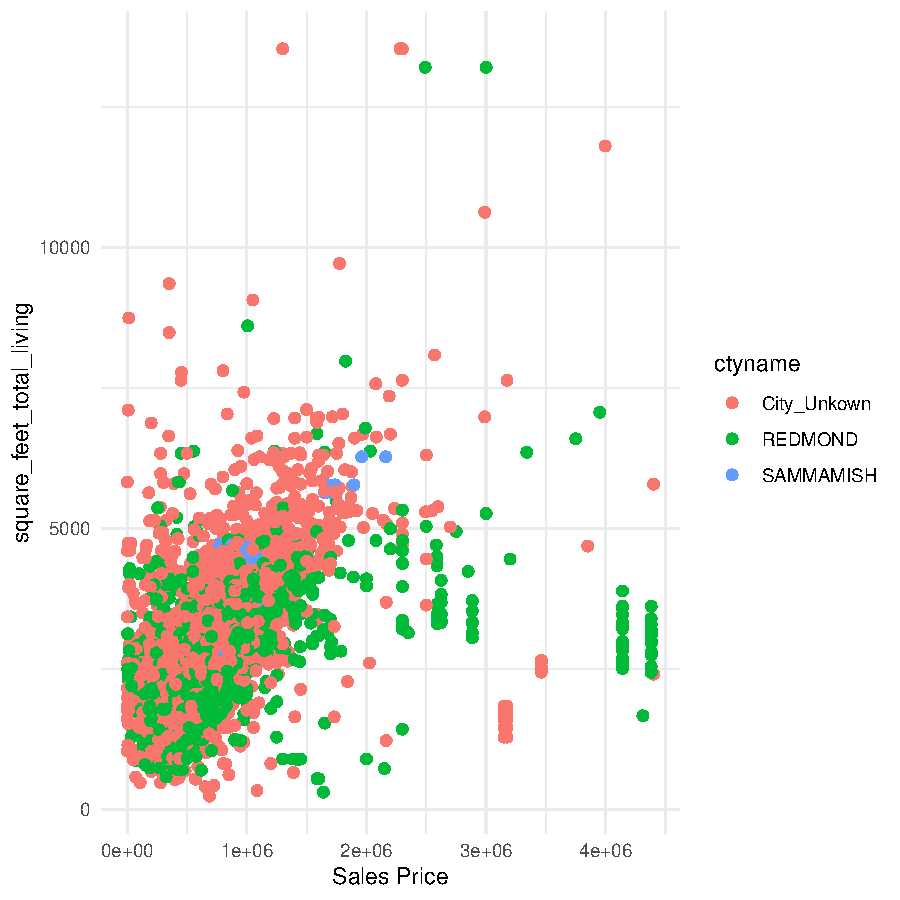
\includegraphics[width=.6\linewidth]{figure/assignment-04-02-Couto-Maria-Rnwauto-report-2} 

}


\begin{kframe}\begin{alltt}
\hlcom{# Create at least 2 new variables}
\hlcom{# Variable/column 1 (Property_Size)}
\hlstd{housedf_v2} \hlkwb{<-} \hlkwd{mutate}\hlstd{(housedf_v2,}\hlkwc{Property_size} \hlstd{=}
                       \hlkwd{cut}\hlstd{(sq_ft_lot,}
                       \hlkwc{breaks} \hlstd{=} \hlkwd{c}\hlstd{(}\hlnum{0}\hlstd{,}\hlnum{10000}\hlstd{,}\hlnum{50000}\hlstd{,}\hlnum{Inf}\hlstd{),}
                       \hlkwc{labels} \hlstd{=} \hlkwd{c}\hlstd{(}\hlstr{"Small"}\hlstd{,}\hlstr{"Medium"}\hlstd{,}\hlstr{"Large"}\hlstd{),}
                                                    \hlkwc{right} \hlstd{=} \hlnum{FALSE}\hlstd{))}
\hlkwd{colnames}\hlstd{(housedf_v2)}
\end{alltt}
\begin{verbatim}
##  [1] "sale_date"                "sale_price"               "sale_reason"             
##  [4] "sale_instrument"          "sale_warning"             "sitetype"                
##  [7] "addr_full"                "zip5"                     "ctyname"                 
## [10] "postalctyn"               "lon"                      "lat"                     
## [13] "building_grade"           "square_feet_total_living" "bedrooms"                
## [16] "bath_full_count"          "bath_half_count"          "bath_3qtr_count"         
## [19] "year_built"               "year_renovated"           "current_zoning"          
## [22] "sq_ft_lot"                "prop_type"                "present_use"             
## [25] "Price_per_sqft"           "Property_size"
\end{verbatim}
\begin{alltt}
\hlkwd{distinct}\hlstd{(housedf_v2,Property_size)}
\end{alltt}
\begin{verbatim}
## # A tibble: 3 x 1
##   Property_size
##   <fct>        
## 1 Small        
## 2 Large        
## 3 Medium
\end{verbatim}
\begin{alltt}
\hlstd{housedf_v2} \hlopt \hlkwd{select}\hlstd{(ctyname,sq_ft_lot,Property_size)}
\end{alltt}
\begin{verbatim}
## # A tibble: 12,865 x 3
##    ctyname     sq_ft_lot Property_size
##    <chr>           <dbl> <fct>        
##  1 REDMOND          6635 Small        
##  2 REDMOND          5570 Small        
##  3 City_Unkown      8444 Small        
##  4 REDMOND          9600 Small        
##  5 REDMOND          7526 Small        
##  6 City_Unkown      7280 Small        
##  7 City_Unkown     97574 Large        
##  8 City_Unkown     30649 Medium       
##  9 City_Unkown     42688 Medium       
## 10 REDMOND         94889 Large        
## # i 12,855 more rows
\end{verbatim}
\begin{alltt}
\hlcom{# Variable/Column 2}

\hlstd{housedf_v2} \hlkwb{<-} \hlkwd{mutate}\hlstd{(housedf_v2,} \hlkwc{Price_Range} \hlstd{=}
                       \hlkwd{cut}\hlstd{(sale_price,}
                           \hlkwc{breaks} \hlstd{=} \hlkwd{c}\hlstd{(}\hlnum{0}\hlstd{,}\hlnum{300000}\hlstd{,}\hlnum{600000}\hlstd{,}\hlnum{Inf}\hlstd{),}
                           \hlkwc{labels} \hlstd{=} \hlkwd{c}\hlstd{(}\hlstr{"Low_Priced"}\hlstd{,}\hlstr{"Medium_Priced"}\hlstd{,}
                                      \hlstr{"High_Priced"}\hlstd{),}\hlkwc{right} \hlstd{=} \hlnum{FALSE}\hlstd{))}
\hlkwd{colnames}\hlstd{(housedf_v2)}
\end{alltt}
\begin{verbatim}
##  [1] "sale_date"                "sale_price"               "sale_reason"             
##  [4] "sale_instrument"          "sale_warning"             "sitetype"                
##  [7] "addr_full"                "zip5"                     "ctyname"                 
## [10] "postalctyn"               "lon"                      "lat"                     
## [13] "building_grade"           "square_feet_total_living" "bedrooms"                
## [16] "bath_full_count"          "bath_half_count"          "bath_3qtr_count"         
## [19] "year_built"               "year_renovated"           "current_zoning"          
## [22] "sq_ft_lot"                "prop_type"                "present_use"             
## [25] "Price_per_sqft"           "Property_size"            "Price_Range"
\end{verbatim}
\begin{alltt}
\hlkwd{distinct}\hlstd{(housedf_v2,Price_Range)}
\end{alltt}
\begin{verbatim}
## # A tibble: 3 x 1
##   Price_Range  
##   <fct>        
## 1 High_Priced  
## 2 Medium_Priced
## 3 Low_Priced
\end{verbatim}
\begin{alltt}
\hlstd{housedf_v2} \hlopt \hlkwd{select}\hlstd{(ctyname,sq_ft_lot,Property_size,Price_Range)}
\end{alltt}
\begin{verbatim}
## # A tibble: 12,865 x 4
##    ctyname     sq_ft_lot Property_size Price_Range  
##    <chr>           <dbl> <fct>         <fct>        
##  1 REDMOND          6635 Small         High_Priced  
##  2 REDMOND          5570 Small         High_Priced  
##  3 City_Unkown      8444 Small         Medium_Priced
##  4 REDMOND          9600 Small         Medium_Priced
##  5 REDMOND          7526 Small         Medium_Priced
##  6 City_Unkown      7280 Small         Low_Priced   
##  7 City_Unkown     97574 Large         High_Priced  
##  8 City_Unkown     30649 Medium        High_Priced  
##  9 City_Unkown     42688 Medium        High_Priced  
## 10 REDMOND         94889 Large         High_Priced  
## # i 12,855 more rows
\end{verbatim}
\end{kframe}
\end{knitrout}

The R session information (including the OS info, R version and all
packages used):

\begin{knitrout}
\definecolor{shadecolor}{rgb}{0.969, 0.969, 0.969}\color{fgcolor}\begin{kframe}
\begin{alltt}
\hlkwd{sessionInfo}\hlstd{()}
\end{alltt}
\begin{verbatim}
## R version 4.3.0 (2023-04-21 ucrt)
## Platform: x86_64-w64-mingw32/x64 (64-bit)
## Running under: Windows 11 x64 (build 22621)
## 
## Matrix products: default
## 
## 
## locale:
## [1] LC_COLLATE=English_United States.utf8  LC_CTYPE=English_United States.utf8   
## [3] LC_MONETARY=English_United States.utf8 LC_NUMERIC=C                          
## [5] LC_TIME=English_United States.utf8    
## 
## time zone: America/New_York
## tzcode source: internal
## 
## attached base packages:
## [1] stats     graphics  grDevices utils     datasets  methods   base     
## 
## other attached packages:
## [1] ggplot2_3.4.2 dplyr_1.1.2   plyr_1.8.8    readxl_1.4.2  RSQLite_2.3.1
## 
## loaded via a namespace (and not attached):
##  [1] bit_4.0.5        gtable_0.3.3     compiler_4.3.0   highr_0.10       tidyselect_1.2.0
##  [6] Rcpp_1.0.10      blob_1.2.4       scales_1.2.1     fastmap_1.1.1    R6_2.5.1        
## [11] labeling_0.4.2   generics_0.1.3   knitr_1.43       tibble_3.2.1     munsell_0.5.0   
## [16] DBI_1.1.3        pillar_1.9.0     rlang_1.1.1      utf8_1.2.3       cachem_1.0.8    
## [21] xfun_0.39        bit64_4.0.5      memoise_2.0.1    cli_3.6.1        withr_2.5.0     
## [26] magrittr_2.0.3   grid_4.3.0       rstudioapi_0.14  lifecycle_1.0.3  vctrs_0.6.2     
## [31] evaluate_0.21    glue_1.6.2       farver_2.1.1     cellranger_1.1.0 fansi_1.0.4     
## [36] colorspace_2.1-0 tools_4.3.0      pkgconfig_2.0.3
\end{verbatim}
\begin{alltt}
\hlkwd{Sys.time}\hlstd{()}
\end{alltt}
\begin{verbatim}
## [1] "2023-07-02 18:48:11 EDT"
\end{verbatim}
\end{kframe}
\end{knitrout}


\end{document}
